% Options for packages loaded elsewhere
\PassOptionsToPackage{unicode}{hyperref}
\PassOptionsToPackage{hyphens}{url}
%
\documentclass[
]{article}
\usepackage{amsmath,amssymb}
\usepackage{lmodern}
\usepackage{iftex}
\ifPDFTeX
  \usepackage[T1]{fontenc}
  \usepackage[utf8]{inputenc}
  \usepackage{textcomp} % provide euro and other symbols
\else % if luatex or xetex
  \usepackage{unicode-math}
  \defaultfontfeatures{Scale=MatchLowercase}
  \defaultfontfeatures[\rmfamily]{Ligatures=TeX,Scale=1}
\fi
% Use upquote if available, for straight quotes in verbatim environments
\IfFileExists{upquote.sty}{\usepackage{upquote}}{}
\IfFileExists{microtype.sty}{% use microtype if available
  \usepackage[]{microtype}
  \UseMicrotypeSet[protrusion]{basicmath} % disable protrusion for tt fonts
}{}
\makeatletter
\@ifundefined{KOMAClassName}{% if non-KOMA class
  \IfFileExists{parskip.sty}{%
    \usepackage{parskip}
  }{% else
    \setlength{\parindent}{0pt}
    \setlength{\parskip}{6pt plus 2pt minus 1pt}}
}{% if KOMA class
  \KOMAoptions{parskip=half}}
\makeatother
\usepackage{xcolor}
\usepackage[margin=1in]{geometry}
\usepackage{color}
\usepackage{fancyvrb}
\newcommand{\VerbBar}{|}
\newcommand{\VERB}{\Verb[commandchars=\\\{\}]}
\DefineVerbatimEnvironment{Highlighting}{Verbatim}{commandchars=\\\{\}}
% Add ',fontsize=\small' for more characters per line
\usepackage{framed}
\definecolor{shadecolor}{RGB}{248,248,248}
\newenvironment{Shaded}{\begin{snugshade}}{\end{snugshade}}
\newcommand{\AlertTok}[1]{\textcolor[rgb]{0.94,0.16,0.16}{#1}}
\newcommand{\AnnotationTok}[1]{\textcolor[rgb]{0.56,0.35,0.01}{\textbf{\textit{#1}}}}
\newcommand{\AttributeTok}[1]{\textcolor[rgb]{0.77,0.63,0.00}{#1}}
\newcommand{\BaseNTok}[1]{\textcolor[rgb]{0.00,0.00,0.81}{#1}}
\newcommand{\BuiltInTok}[1]{#1}
\newcommand{\CharTok}[1]{\textcolor[rgb]{0.31,0.60,0.02}{#1}}
\newcommand{\CommentTok}[1]{\textcolor[rgb]{0.56,0.35,0.01}{\textit{#1}}}
\newcommand{\CommentVarTok}[1]{\textcolor[rgb]{0.56,0.35,0.01}{\textbf{\textit{#1}}}}
\newcommand{\ConstantTok}[1]{\textcolor[rgb]{0.00,0.00,0.00}{#1}}
\newcommand{\ControlFlowTok}[1]{\textcolor[rgb]{0.13,0.29,0.53}{\textbf{#1}}}
\newcommand{\DataTypeTok}[1]{\textcolor[rgb]{0.13,0.29,0.53}{#1}}
\newcommand{\DecValTok}[1]{\textcolor[rgb]{0.00,0.00,0.81}{#1}}
\newcommand{\DocumentationTok}[1]{\textcolor[rgb]{0.56,0.35,0.01}{\textbf{\textit{#1}}}}
\newcommand{\ErrorTok}[1]{\textcolor[rgb]{0.64,0.00,0.00}{\textbf{#1}}}
\newcommand{\ExtensionTok}[1]{#1}
\newcommand{\FloatTok}[1]{\textcolor[rgb]{0.00,0.00,0.81}{#1}}
\newcommand{\FunctionTok}[1]{\textcolor[rgb]{0.00,0.00,0.00}{#1}}
\newcommand{\ImportTok}[1]{#1}
\newcommand{\InformationTok}[1]{\textcolor[rgb]{0.56,0.35,0.01}{\textbf{\textit{#1}}}}
\newcommand{\KeywordTok}[1]{\textcolor[rgb]{0.13,0.29,0.53}{\textbf{#1}}}
\newcommand{\NormalTok}[1]{#1}
\newcommand{\OperatorTok}[1]{\textcolor[rgb]{0.81,0.36,0.00}{\textbf{#1}}}
\newcommand{\OtherTok}[1]{\textcolor[rgb]{0.56,0.35,0.01}{#1}}
\newcommand{\PreprocessorTok}[1]{\textcolor[rgb]{0.56,0.35,0.01}{\textit{#1}}}
\newcommand{\RegionMarkerTok}[1]{#1}
\newcommand{\SpecialCharTok}[1]{\textcolor[rgb]{0.00,0.00,0.00}{#1}}
\newcommand{\SpecialStringTok}[1]{\textcolor[rgb]{0.31,0.60,0.02}{#1}}
\newcommand{\StringTok}[1]{\textcolor[rgb]{0.31,0.60,0.02}{#1}}
\newcommand{\VariableTok}[1]{\textcolor[rgb]{0.00,0.00,0.00}{#1}}
\newcommand{\VerbatimStringTok}[1]{\textcolor[rgb]{0.31,0.60,0.02}{#1}}
\newcommand{\WarningTok}[1]{\textcolor[rgb]{0.56,0.35,0.01}{\textbf{\textit{#1}}}}
\usepackage{graphicx}
\makeatletter
\def\maxwidth{\ifdim\Gin@nat@width>\linewidth\linewidth\else\Gin@nat@width\fi}
\def\maxheight{\ifdim\Gin@nat@height>\textheight\textheight\else\Gin@nat@height\fi}
\makeatother
% Scale images if necessary, so that they will not overflow the page
% margins by default, and it is still possible to overwrite the defaults
% using explicit options in \includegraphics[width, height, ...]{}
\setkeys{Gin}{width=\maxwidth,height=\maxheight,keepaspectratio}
% Set default figure placement to htbp
\makeatletter
\def\fps@figure{htbp}
\makeatother
\setlength{\emergencystretch}{3em} % prevent overfull lines
\providecommand{\tightlist}{%
  \setlength{\itemsep}{0pt}\setlength{\parskip}{0pt}}
\setcounter{secnumdepth}{-\maxdimen} % remove section numbering
\ifLuaTeX
  \usepackage{selnolig}  % disable illegal ligatures
\fi
\IfFileExists{bookmark.sty}{\usepackage{bookmark}}{\usepackage{hyperref}}
\IfFileExists{xurl.sty}{\usepackage{xurl}}{} % add URL line breaks if available
\urlstyle{same} % disable monospaced font for URLs
\hypersetup{
  pdftitle={UROP Final Report},
  pdfauthor={Emi Cervantes, Sophia Ma},
  hidelinks,
  pdfcreator={LaTeX via pandoc}}

\title{UROP Final Report}
\author{Emi Cervantes, Sophia Ma}
\date{2023-05-16}

\begin{document}
\maketitle

\hypertarget{abstract}{%
\section{Abstract}\label{abstract}}

Cognitive Load Theory (Sweller, 2011) suggests that worked examples,
mathematical problems with written out solutions, can increase students'
available working memory resources - which are a limited set of
cognitive attention resources that allow students to learn mathematics
concepts and solve word problems. Worked examples may offload attention
to written word problem solutions rather than requiring learners to hold
them in mind, creating more efficient learning. At the same time, many
students feel mathematical anxiety when faced with mathematics learning
and problem solving, which can generate worries that engage the same
limited set of working memory resources, reducing available resources
for new learning and problem solving. To test whether worked examples
could mitigate the deleterious effects of mathematical anxiety on
performance, a pre-post design experiment was conducted on 280
fifth-graders from ten schools in Orange County and Chicago to see
whether worked examples could reduce mathematical anxiety in students
learning ratios - a challenging mathematical concept. The study also
examined other potential relationships with mathematical anxiety such as
mind wandering and situational interest. A multiple linear regression
model was used to assess the relationships between these key features.
Findings indicate that for those who were given worked examples during
instruction, their mathematical anxiety was mitigated which allowed them
to perform more accurately in the delayed assessment. Mathematical
anxiety was a significant predictor of mind wandering, which is a factor
in predicting students' performance as well.

\hypertarget{study-summary}{%
\section{Study Summary}\label{study-summary}}

\begin{itemize}
\item
  280 fifth-graders from 10 schools, 8 in Orange County, California and
  2 in Chicago, Illinois
\item
  \textbf{Pre-post design experiment:} students were given a 20-minute
  video lesson on ratios on day 1

  \begin{itemize}
  \item
    Experimental group: worked examples present
  \item
    Control group: no worked examples provided
  \end{itemize}
\item
  \textbf{Post-study} (3 days after day 1): Students completed math
  anxiety questionnaire (TMA) and post-test assessing their ratio
  knowledge
\end{itemize}

\hypertarget{load-libraries}{%
\section{Load Libraries}\label{load-libraries}}

\begin{Shaded}
\begin{Highlighting}[]
\FunctionTok{library}\NormalTok{(tidyverse)}
\end{Highlighting}
\end{Shaded}

\begin{verbatim}
## -- Attaching core tidyverse packages ------------------------ tidyverse 2.0.0 --
## v dplyr     1.1.2     v readr     2.1.4
## v forcats   1.0.0     v stringr   1.5.0
## v ggplot2   3.4.2     v tibble    3.2.1
## v lubridate 1.9.2     v tidyr     1.3.0
## v purrr     1.0.1     
## -- Conflicts ------------------------------------------ tidyverse_conflicts() --
## x dplyr::filter() masks stats::filter()
## x dplyr::lag()    masks stats::lag()
## i Use the ]8;;http://conflicted.r-lib.org/conflicted package]8;; to force all conflicts to become errors
\end{verbatim}

\begin{Shaded}
\begin{Highlighting}[]
\FunctionTok{library}\NormalTok{(gridExtra)}
\end{Highlighting}
\end{Shaded}

\begin{verbatim}
## 
## Attaching package: 'gridExtra'
## 
## The following object is masked from 'package:dplyr':
## 
##     combine
\end{verbatim}

\begin{Shaded}
\begin{Highlighting}[]
\FunctionTok{library}\NormalTok{(ggpubr)}
\end{Highlighting}
\end{Shaded}

\hypertarget{load-data}{%
\section{Load Data}\label{load-data}}

\begin{Shaded}
\begin{Highlighting}[]
\NormalTok{dfr }\OtherTok{\textless{}{-}}\NormalTok{ readxl}\SpecialCharTok{::}\FunctionTok{read\_xlsx}\NormalTok{(}\StringTok{"../data/KidsCOVID\_Winter21\_raw data.xlsx"}\NormalTok{)}
\end{Highlighting}
\end{Shaded}

\begin{verbatim}
## New names:
## * `Subject ID #` -> `Subject ID #...8`
## * `Subject ID #` -> `Subject ID #...9`
## * `StartDate` -> `StartDate...11`
## * `EndDate` -> `EndDate...12`
## * `Progress` -> `Progress...13`
## * `Duration (in seconds)` -> `Duration (in seconds)...17`
## * `Finished` -> `Finished...18`
## * `RecordedDate` -> `RecordedDate...19`
## * `Browser_info_Browser` -> `Browser_info_Browser...20`
## * `Browser_info_Version` -> `Browser_info_Version...21`
## * `Browser_info_Operating System` -> `Browser_info_Operating System...22`
## * `Browser_info_Resolution` -> `Browser_info_Resolution...23`
## * `Misc_0` -> `Misc_0...36`
## * `Misc_1` -> `Misc_1...100`
## * `Misc_2` -> `Misc_2...145`
## * `MW_control_1` -> `MW_control_1...210`
## * `MW_control_2` -> `MW_control_2...211`
## * `MW_control_3` -> `MW_control_3...212`
## * `MW_control_4` -> `MW_control_4...213`
## * `MW_control_5` -> `MW_control_5...214`
## * `` -> `...219`
## * `StartDate` -> `StartDate...221`
## * `EndDate` -> `EndDate...222`
## * `Progress` -> `Progress...223`
## * `Duration (in seconds)` -> `Duration (in seconds)...224`
## * `Finished` -> `Finished...225`
## * `RecordedDate` -> `RecordedDate...226`
## * `Browser_info_Browser` -> `Browser_info_Browser...227`
## * `Browser_info_Version` -> `Browser_info_Version...228`
## * `Browser_info_Operating System` -> `Browser_info_Operating System...229`
## * `Browser_info_Resolution` -> `Browser_info_Resolution...230`
## * `Misc_0` -> `Misc_0...232`
## * `Misc_1` -> `Misc_1...239`
## * `Misc_2` -> `Misc_2...290`
## * `MW_control_1` -> `MW_control_1...295`
## * `MW_control_2` -> `MW_control_2...296`
## * `MW_control_3` -> `MW_control_3...297`
## * `MW_control_4` -> `MW_control_4...298`
## * `MW_control_5` -> `MW_control_5...299`
\end{verbatim}

\begin{Shaded}
\begin{Highlighting}[]
\CommentTok{\# Number of rows in dfr}
\FunctionTok{nrow}\NormalTok{(dfr)}
\end{Highlighting}
\end{Shaded}

\begin{verbatim}
## [1] 303
\end{verbatim}

\begin{Shaded}
\begin{Highlighting}[]
\CommentTok{\# Number of columns in dfr}
\FunctionTok{ncol}\NormalTok{(dfr)}
\end{Highlighting}
\end{Shaded}

\begin{verbatim}
## [1] 409
\end{verbatim}

The raw data contains 299 students' data and 410 vairables

\hypertarget{data-cleaning}{%
\section{Data Cleaning}\label{data-cleaning}}

We first noticed that some students from the data were not assigned to
any group (NA):

\begin{Shaded}
\begin{Highlighting}[]
\NormalTok{dfr }\SpecialCharTok{\%\textgreater{}\%} \FunctionTok{ggplot}\NormalTok{(}\FunctionTok{aes}\NormalTok{(}\AttributeTok{x =}\NormalTok{ Condition, }\AttributeTok{fill =}\NormalTok{ Condition)) }\SpecialCharTok{+} 
  \FunctionTok{geom\_bar}\NormalTok{(}\AttributeTok{color =} \StringTok{"black"}\NormalTok{) }\SpecialCharTok{+} \FunctionTok{theme\_minimal}\NormalTok{() }\SpecialCharTok{+}
  \FunctionTok{labs}\NormalTok{(}\AttributeTok{title =} \StringTok{"Study Conditions"}\NormalTok{)}
\end{Highlighting}
\end{Shaded}

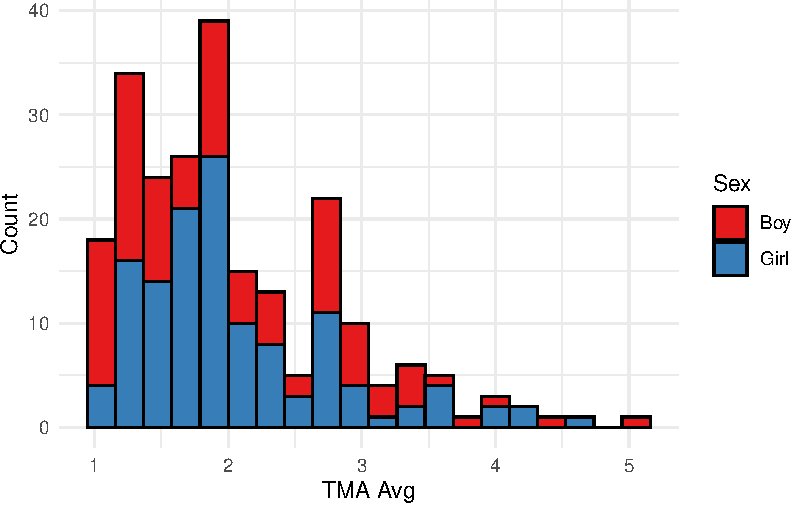
\includegraphics{urop_final_report_files/figure-latex/unnamed-chunk-3-1.pdf}

We want to look at \emph{no worked example} and \emph{worked example}
group, so we removed all the data without condition. The raw data
assigned \texttt{Condition} = 1 is for students in \emph{worked example}
group, and \texttt{Condition} = 2 for students in \emph{no worked
example} group. For clear readability, we assigned 0 to all students in
\emph{no worked example} group:

\begin{Shaded}
\begin{Highlighting}[]
\CommentTok{\# removing NA condition data}
\NormalTok{dfr }\OtherTok{\textless{}{-}}\NormalTok{dfr }\SpecialCharTok{\%\textgreater{}\%} \FunctionTok{filter}\NormalTok{(Condition }\SpecialCharTok{==} \DecValTok{1} \SpecialCharTok{|}\NormalTok{ Condition }\SpecialCharTok{==} \DecValTok{2}\NormalTok{)}
\CommentTok{\# assigning 0 to no worked example group data}
\NormalTok{dfr}\SpecialCharTok{$}\NormalTok{Condition[dfr}\SpecialCharTok{$}\NormalTok{Condition }\SpecialCharTok{==} \DecValTok{2}\NormalTok{] }\OtherTok{=} \DecValTok{0} 
\end{Highlighting}
\end{Shaded}

For our UROP project, we are interested in comparing the effects of math
anxiety (\texttt{TMA\_avg}) on students' accuracy scores
(\texttt{Del\_OverallAcc}) between the worked example and no worked
example groups. Furthermore, we are interested in observing the impacts
of other factors from data such as mind wandering scores
(\texttt{mw\_avg}) and situational interest (\texttt{SI\_avg}).

\begin{Shaded}
\begin{Highlighting}[]
\CommentTok{\# Get the average of mw\_1 and mw\_2}
\NormalTok{dfr }\OtherTok{\textless{}{-}}\NormalTok{ dfr }\SpecialCharTok{\%\textgreater{}\%} \FunctionTok{mutate}\NormalTok{(}\AttributeTok{mw\_avg =} \FunctionTok{rowMeans}\NormalTok{(dfr[}\DecValTok{346}\SpecialCharTok{:}\DecValTok{347}\NormalTok{], }\AttributeTok{na.rm =} \ConstantTok{TRUE}\NormalTok{))}
\CommentTok{\# Select columns and remove any row with missing data}
\NormalTok{df }\OtherTok{\textless{}{-}}\NormalTok{ dfr }\SpecialCharTok{\%\textgreater{}\%} \FunctionTok{select}\NormalTok{(Del\_OverallAcc, TMA\_avg, Condition, mw\_avg, SI\_avg) }\SpecialCharTok{\%\textgreater{}\%} 
  \FunctionTok{drop\_na}\NormalTok{()}
\FunctionTok{glimpse}\NormalTok{(df)}
\end{Highlighting}
\end{Shaded}

\begin{verbatim}
## Rows: 229
## Columns: 5
## $ Del_OverallAcc <dbl> 0.3666667, 0.9000000, 0.5000000, 0.6000000, 0.1666667, ~
## $ TMA_avg        <dbl> 1.833333, 2.000000, 2.166667, 1.666667, 2.000000, 1.666~
## $ Condition      <chr> "1", "1", "1", "1", "0", "1", "1", "0", "0", "0", "1", ~
## $ mw_avg         <dbl> 1.9, 1.9, 2.3, 2.0, 1.5, 1.2, 2.1, 1.2, 2.6, 1.1, 1.2, ~
## $ SI_avg         <dbl> 4.500000, 3.000000, 3.250000, 4.500000, 4.750000, 4.583~
\end{verbatim}

The new data contains 229 students' data and 5 variables

\hypertarget{visualizations}{%
\section{Visualizations}\label{visualizations}}

\hypertarget{math-anxiety-distributions}{%
\subsection{Math Anxiety
Distributions}\label{math-anxiety-distributions}}

\begin{Shaded}
\begin{Highlighting}[]
\CommentTok{\# New facet label names for supp variable}
\NormalTok{cond.labs }\OtherTok{\textless{}{-}} \FunctionTok{c}\NormalTok{(}\StringTok{"No Worked EX"}\NormalTok{, }\StringTok{"Worked EX"}\NormalTok{)}
\FunctionTok{names}\NormalTok{(cond.labs) }\OtherTok{\textless{}{-}} \FunctionTok{c}\NormalTok{(}\DecValTok{0}\NormalTok{, }\DecValTok{1}\NormalTok{)}
\CommentTok{\# Histogram of tma\_avg }
\NormalTok{df }\SpecialCharTok{\%\textgreater{}\%} 
  \FunctionTok{ggplot}\NormalTok{(}\FunctionTok{aes}\NormalTok{(}\AttributeTok{x =}\NormalTok{ TMA\_avg, }\AttributeTok{fill =}\NormalTok{ Condition)) }\SpecialCharTok{+} 
  \FunctionTok{geom\_histogram}\NormalTok{(}\AttributeTok{color =} \StringTok{"black"}\NormalTok{, }\AttributeTok{bins =} \DecValTok{20}\NormalTok{) }\SpecialCharTok{+}
  \FunctionTok{theme\_minimal}\NormalTok{()}\SpecialCharTok{+} 
  \FunctionTok{scale\_fill\_manual}\NormalTok{(}\AttributeTok{values =} \FunctionTok{c}\NormalTok{(}\StringTok{"\#ef476f"}\NormalTok{,}\StringTok{"\#1b9aaa"}\NormalTok{), }\AttributeTok{labels =} \FunctionTok{c}\NormalTok{(}\StringTok{"No Worked EX"}\NormalTok{, }\StringTok{"Worked EX"}\NormalTok{)) }\SpecialCharTok{+}
  \FunctionTok{facet\_grid}\NormalTok{(.}\SpecialCharTok{\textasciitilde{}}\NormalTok{Condition, }\AttributeTok{labeller =} \FunctionTok{labeller}\NormalTok{(}\AttributeTok{Condition =}\NormalTok{ cond.labs))  }\SpecialCharTok{+}
  \FunctionTok{labs}\NormalTok{(}\AttributeTok{title =} \StringTok{"Math Anxiety Distributions"}\NormalTok{, }\AttributeTok{x =} \StringTok{"TMA Average"}\NormalTok{)}
\end{Highlighting}
\end{Shaded}

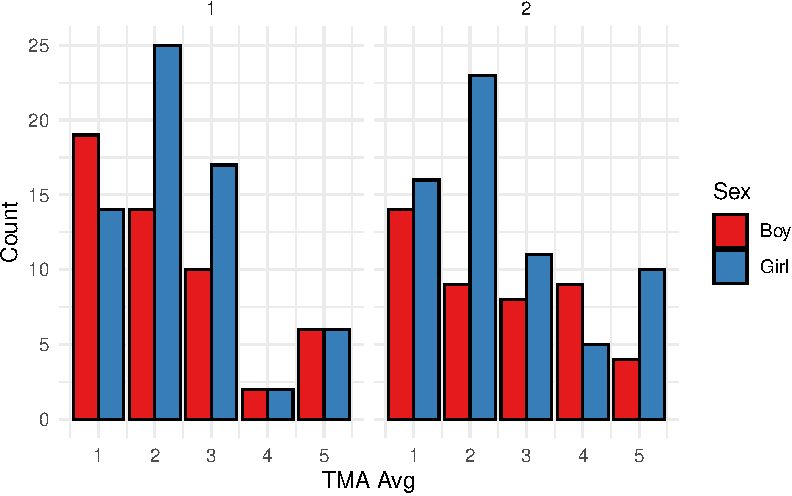
\includegraphics{urop_final_report_files/figure-latex/unnamed-chunk-6-1.pdf}

For both groups, the distributions seemed to be right-skewed, indicating
that the average math anxiety was low for both groups:

\begin{Shaded}
\begin{Highlighting}[]
\CommentTok{\# table summary of math anxiety}
\NormalTok{df }\SpecialCharTok{\%\textgreater{}\%} 
  \FunctionTok{group\_by}\NormalTok{(Condition) }\SpecialCharTok{\%\textgreater{}\%} 
  \FunctionTok{summarize}\NormalTok{(}\StringTok{"Average TMA"} \OtherTok{=} \FunctionTok{mean}\NormalTok{(TMA\_avg), }\StringTok{"Standard deviation"} \OtherTok{=} \FunctionTok{sd}\NormalTok{(TMA\_avg))}
\end{Highlighting}
\end{Shaded}

\begin{verbatim}
## # A tibble: 2 x 3
##   Condition `Average TMA` `Standard deviation`
##   <chr>             <dbl>                <dbl>
## 1 0                  2.09                0.832
## 2 1                  1.99                0.762
\end{verbatim}

\begin{Shaded}
\begin{Highlighting}[]
\CommentTok{\# Math anxiety average bar plot}
\NormalTok{df }\SpecialCharTok{\%\textgreater{}\%} 
  \FunctionTok{group\_by}\NormalTok{(Condition) }\SpecialCharTok{\%\textgreater{}\%} 
  \FunctionTok{summarize}\NormalTok{(}\AttributeTok{tma\_avg =} \FunctionTok{mean}\NormalTok{(TMA\_avg))  }\SpecialCharTok{\%\textgreater{}\%} 
  \FunctionTok{ggplot}\NormalTok{(}\FunctionTok{aes}\NormalTok{(}\AttributeTok{x =}\NormalTok{ Condition, }\AttributeTok{y =}\NormalTok{ tma\_avg, }\AttributeTok{fill =}\NormalTok{ Condition)) }\SpecialCharTok{+}
  \FunctionTok{geom\_bar}\NormalTok{(}\AttributeTok{position=}\StringTok{"dodge"}\NormalTok{, }\AttributeTok{stat=}\StringTok{"identity"}\NormalTok{) }\SpecialCharTok{+} \FunctionTok{theme\_bw}\NormalTok{() }\SpecialCharTok{+} 
  \FunctionTok{scale\_x\_discrete}\NormalTok{(}\AttributeTok{breaks=}\FunctionTok{c}\NormalTok{(}\DecValTok{0}\NormalTok{,}\DecValTok{1}\NormalTok{),}
        \AttributeTok{labels=}\FunctionTok{c}\NormalTok{(}\StringTok{"No Worked EX"}\NormalTok{,}\StringTok{"Worked EX"}\NormalTok{)) }\SpecialCharTok{+}
  \FunctionTok{scale\_fill\_manual}\NormalTok{(}\AttributeTok{values =} \FunctionTok{c}\NormalTok{(}\StringTok{"\#ef476f"}\NormalTok{,}\StringTok{"\#1b9aaa"}\NormalTok{), }\AttributeTok{labels =} 
                                  \FunctionTok{c}\NormalTok{(}\StringTok{"No Worked EX"}\NormalTok{, }\StringTok{"Worked EX"}\NormalTok{)) }\SpecialCharTok{+}
  \FunctionTok{labs}\NormalTok{(}\AttributeTok{x =} \StringTok{"Condition"}\NormalTok{, }\AttributeTok{y =} \StringTok{"TMA"}\NormalTok{, }\AttributeTok{title =} \StringTok{"Average Math Anxiety Scores"}\NormalTok{)}\SpecialCharTok{+} \FunctionTok{ylim}\NormalTok{(}\DecValTok{0}\NormalTok{,}\DecValTok{5}\NormalTok{)}
\end{Highlighting}
\end{Shaded}

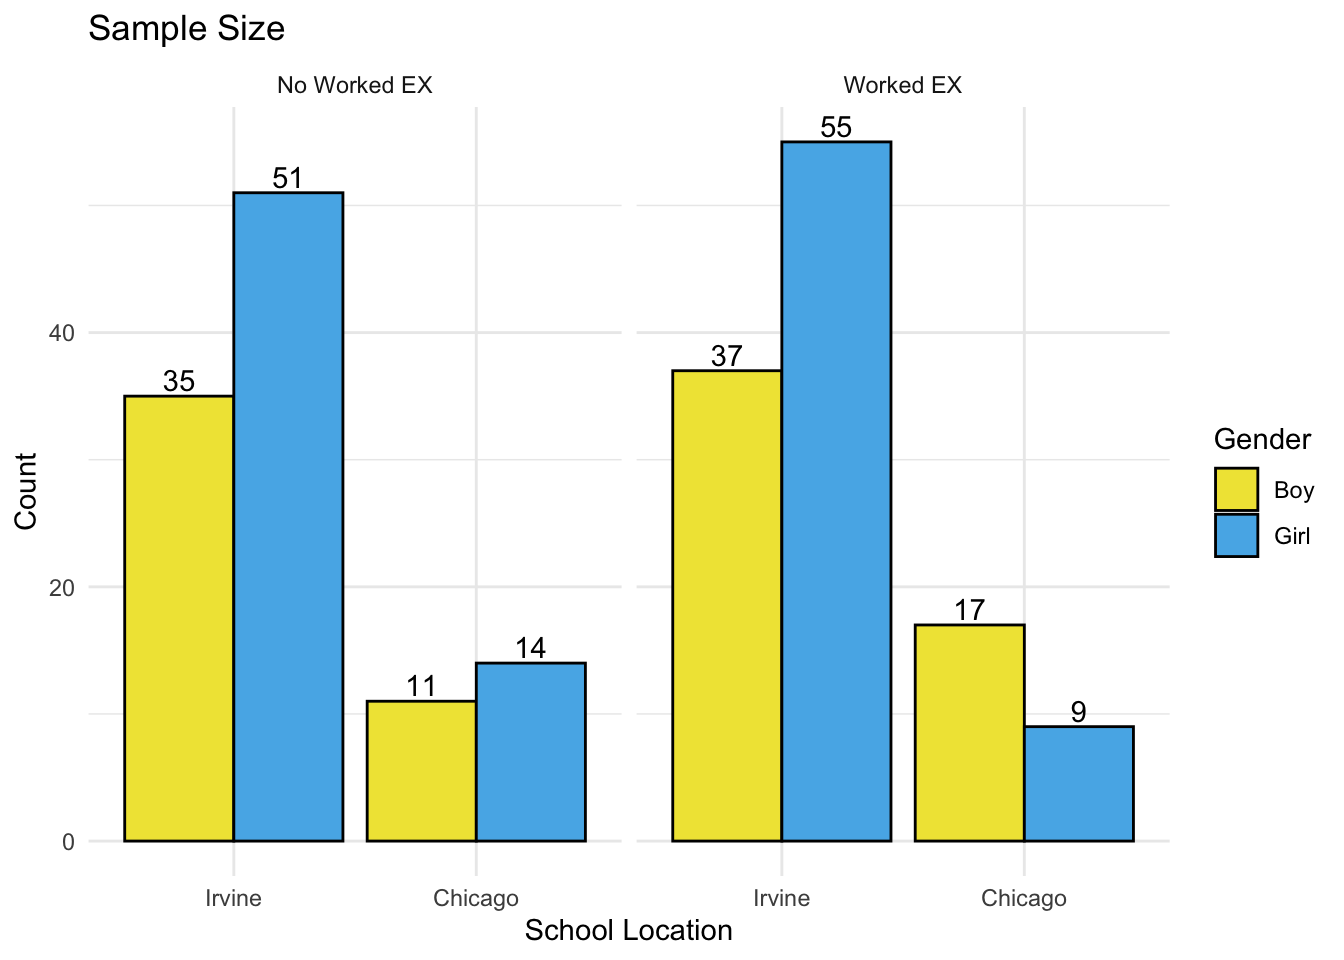
\includegraphics{urop_final_report_files/figure-latex/unnamed-chunk-7-1.pdf}

\hypertarget{post-test-accuracy-score-distributions}{%
\subsection{Post-test accuracy score
distributions}\label{post-test-accuracy-score-distributions}}

\begin{Shaded}
\begin{Highlighting}[]
\CommentTok{\# histogram of post{-}assessment accuracy score}
\NormalTok{df }\SpecialCharTok{\%\textgreater{}\%} 
  \FunctionTok{ggplot}\NormalTok{(}\FunctionTok{aes}\NormalTok{(}\AttributeTok{x =}\NormalTok{ Del\_OverallAcc, }\AttributeTok{fill =}\NormalTok{ Condition)) }\SpecialCharTok{+}
  \FunctionTok{geom\_histogram}\NormalTok{(}\AttributeTok{color =} \StringTok{"black"}\NormalTok{, }\AttributeTok{bins =} \DecValTok{20}\NormalTok{) }\SpecialCharTok{+}
  \FunctionTok{theme\_minimal}\NormalTok{()}\SpecialCharTok{+} 
  \FunctionTok{scale\_fill\_manual}\NormalTok{(}\AttributeTok{values =} \FunctionTok{c}\NormalTok{(}\StringTok{"\#ef476f"}\NormalTok{,}\StringTok{"\#1b9aaa"}\NormalTok{), }\AttributeTok{labels =} \FunctionTok{c}\NormalTok{(}\StringTok{"No Worked EX"}\NormalTok{, }\StringTok{"Worked EX"}\NormalTok{)) }\SpecialCharTok{+}
  \FunctionTok{facet\_grid}\NormalTok{(.}\SpecialCharTok{\textasciitilde{}}\NormalTok{Condition, }\AttributeTok{labeller =} \FunctionTok{labeller}\NormalTok{(}\AttributeTok{Condition =}\NormalTok{ cond.labs))  }\SpecialCharTok{+}
  \FunctionTok{labs}\NormalTok{(}\AttributeTok{title =} \StringTok{"Post{-}Test Accuracy Distributions"}\NormalTok{, }\AttributeTok{x =} \StringTok{"Overall Accuracy"}\NormalTok{)}
\end{Highlighting}
\end{Shaded}

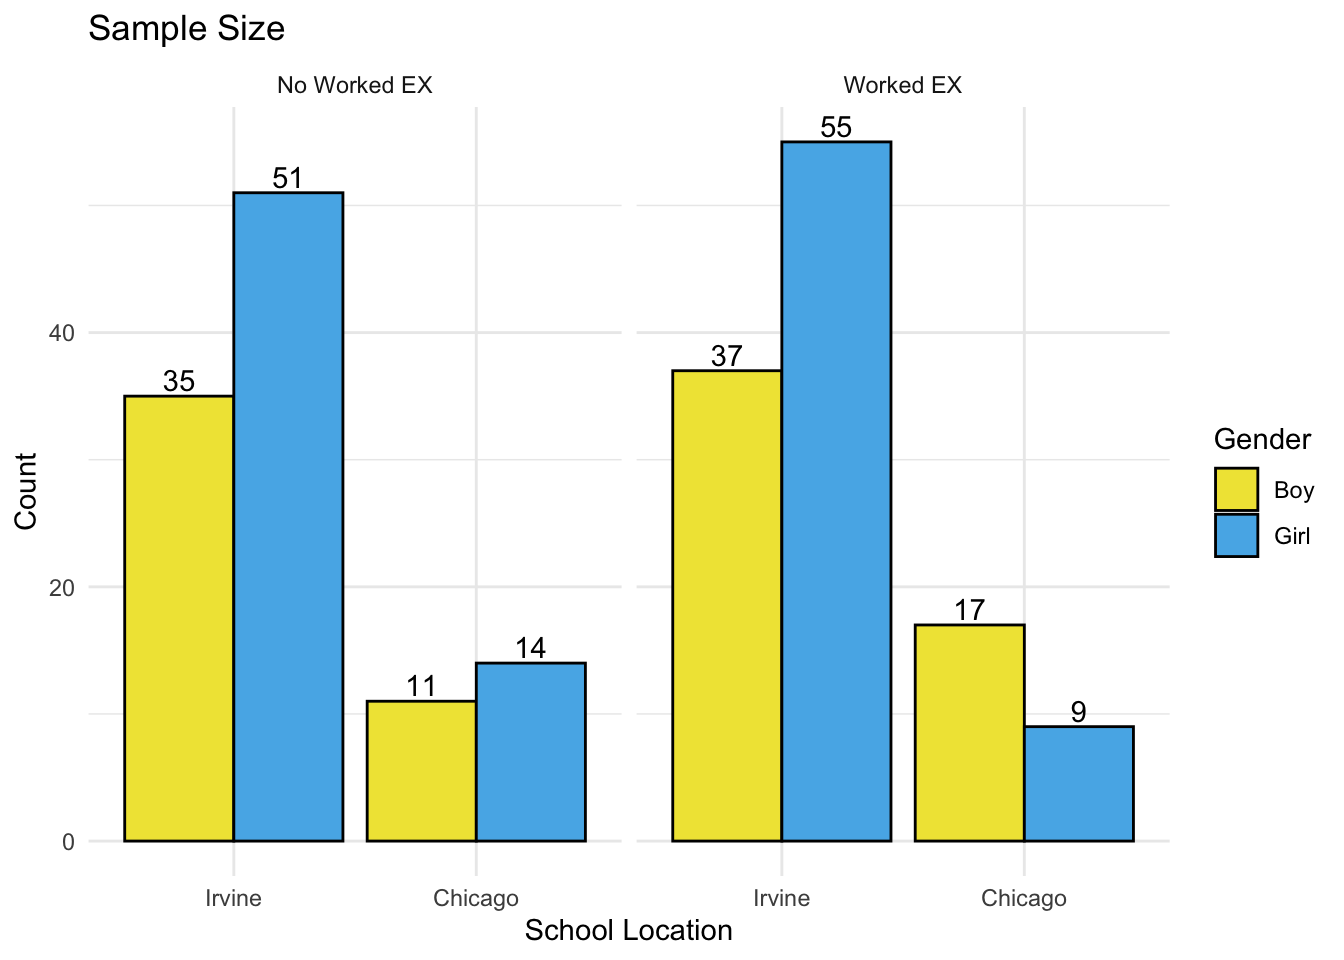
\includegraphics{urop_final_report_files/figure-latex/unnamed-chunk-8-1.pdf}

The averages of post-test accuracy seem to be close for both groups:

\begin{Shaded}
\begin{Highlighting}[]
\CommentTok{\# table summary of accuracy}
\NormalTok{df }\SpecialCharTok{\%\textgreater{}\%} 
  \FunctionTok{group\_by}\NormalTok{(Condition) }\SpecialCharTok{\%\textgreater{}\%} 
  \FunctionTok{summarize}\NormalTok{(}\StringTok{"Average Accuracy"} \OtherTok{=} \FunctionTok{mean}\NormalTok{(Del\_OverallAcc), }\StringTok{"Standard deviation"} \OtherTok{=} \FunctionTok{sd}\NormalTok{(Del\_OverallAcc))}
\end{Highlighting}
\end{Shaded}

\begin{verbatim}
## # A tibble: 2 x 3
##   Condition `Average Accuracy` `Standard deviation`
##   <chr>                  <dbl>                <dbl>
## 1 0                      0.610                0.239
## 2 1                      0.627                0.214
\end{verbatim}

\begin{Shaded}
\begin{Highlighting}[]
\CommentTok{\# test accuracy average bar plot}
\NormalTok{df }\SpecialCharTok{\%\textgreater{}\%} 
  \FunctionTok{group\_by}\NormalTok{(Condition) }\SpecialCharTok{\%\textgreater{}\%} 
  \FunctionTok{summarize}\NormalTok{(}\AttributeTok{acc\_avg =} \FunctionTok{mean}\NormalTok{(Del\_OverallAcc))  }\SpecialCharTok{\%\textgreater{}\%} 
  \FunctionTok{ggplot}\NormalTok{(}\FunctionTok{aes}\NormalTok{(}\AttributeTok{x =}\NormalTok{ Condition, }\AttributeTok{y =}\NormalTok{ acc\_avg, }\AttributeTok{fill =}\NormalTok{ Condition)) }\SpecialCharTok{+}
  \FunctionTok{geom\_bar}\NormalTok{(}\AttributeTok{position=}\StringTok{"dodge"}\NormalTok{, }\AttributeTok{stat=}\StringTok{"identity"}\NormalTok{) }\SpecialCharTok{+} \FunctionTok{theme\_bw}\NormalTok{() }\SpecialCharTok{+} 
  \FunctionTok{scale\_x\_discrete}\NormalTok{(}\AttributeTok{breaks=}\FunctionTok{c}\NormalTok{(}\DecValTok{0}\NormalTok{,}\DecValTok{1}\NormalTok{),}
        \AttributeTok{labels=}\FunctionTok{c}\NormalTok{(}\StringTok{"No Worked EX"}\NormalTok{,}\StringTok{"Worked EX"}\NormalTok{)) }\SpecialCharTok{+}
  \FunctionTok{scale\_fill\_manual}\NormalTok{(}\AttributeTok{values =} \FunctionTok{c}\NormalTok{(}\StringTok{"\#ef476f"}\NormalTok{,}\StringTok{"\#1b9aaa"}\NormalTok{), }\AttributeTok{labels =} 
                                  \FunctionTok{c}\NormalTok{(}\StringTok{"No Worked EX"}\NormalTok{, }\StringTok{"Worked EX"}\NormalTok{)) }\SpecialCharTok{+}
  \FunctionTok{labs}\NormalTok{(}\AttributeTok{x =} \StringTok{"Condition"}\NormalTok{, }\AttributeTok{y =} \StringTok{"TMA"}\NormalTok{, }\AttributeTok{title =} \StringTok{"Post{-}Test Overall Accuracy Scores"}\NormalTok{) }\SpecialCharTok{+} \FunctionTok{ylim}\NormalTok{(}\DecValTok{0}\NormalTok{,}\DecValTok{1}\NormalTok{)}
\end{Highlighting}
\end{Shaded}

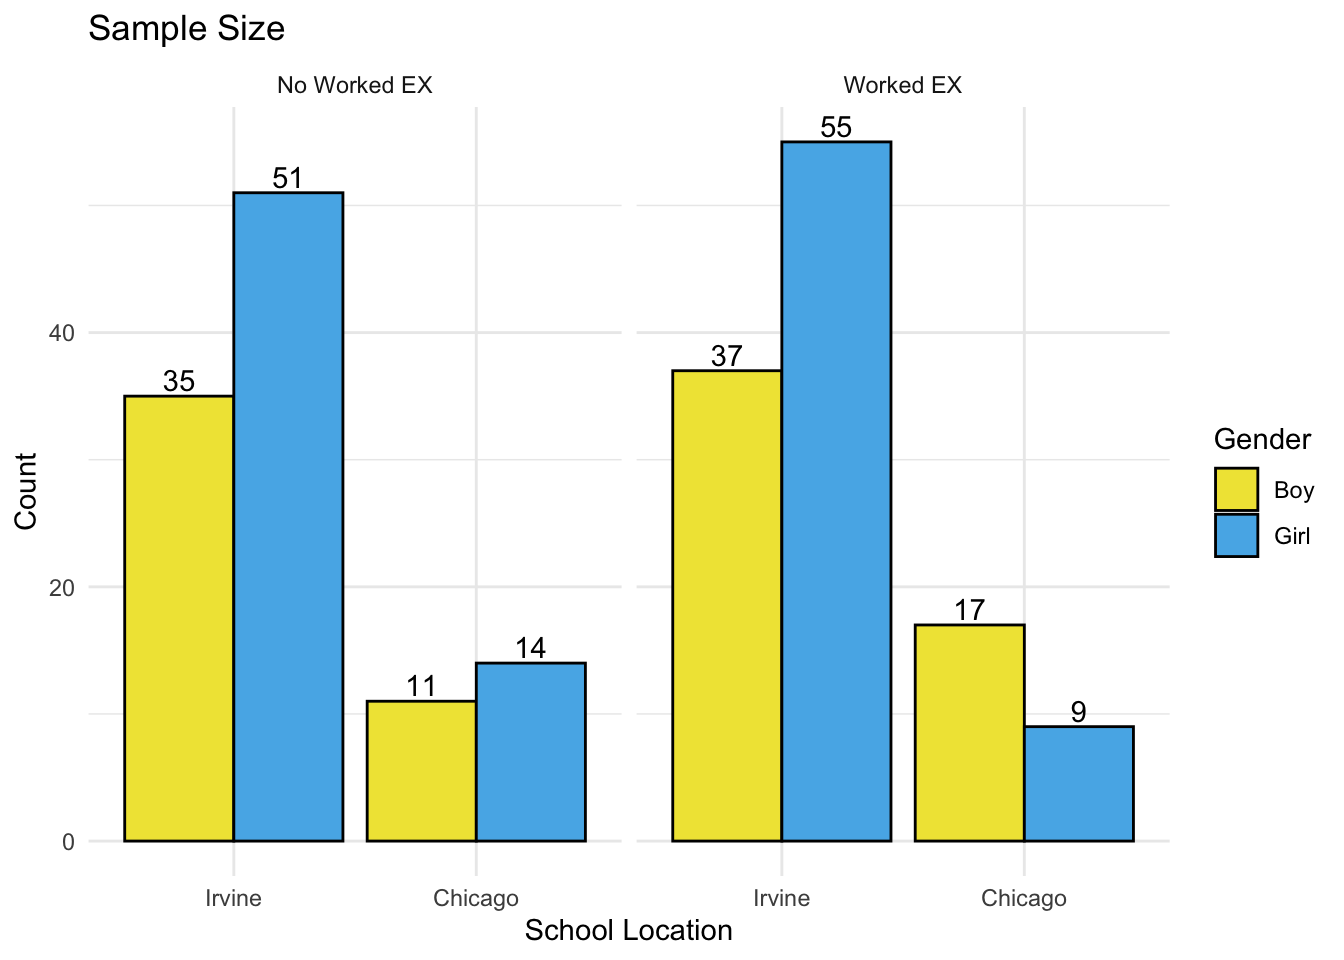
\includegraphics{urop_final_report_files/figure-latex/unnamed-chunk-9-1.pdf}

\hypertarget{relationship-between-math-anxiety-and-overall-accuracy}{%
\subsection{Relationship between math anxiety and overall
accuracy}\label{relationship-between-math-anxiety-and-overall-accuracy}}

\begin{Shaded}
\begin{Highlighting}[]
\CommentTok{\# Scatterplot: tma vs accuracy}
\NormalTok{df }\SpecialCharTok{\%\textgreater{}\%} 
  \FunctionTok{ggplot}\NormalTok{(}\FunctionTok{aes}\NormalTok{(}\AttributeTok{x =}\NormalTok{ TMA\_avg, }\AttributeTok{y =}\NormalTok{ Del\_OverallAcc ,}\AttributeTok{color  =}\NormalTok{ Condition)) }\SpecialCharTok{+} 
  \FunctionTok{geom\_point}\NormalTok{() }\SpecialCharTok{+}
  \FunctionTok{geom\_smooth}\NormalTok{(}\AttributeTok{method =} \StringTok{"lm"}\NormalTok{, }\AttributeTok{se =} \ConstantTok{FALSE}\NormalTok{) }\SpecialCharTok{+}
  \FunctionTok{theme\_bw}\NormalTok{() }\SpecialCharTok{+} 
  \FunctionTok{scale\_color\_manual}\NormalTok{(}\AttributeTok{values =} \FunctionTok{c}\NormalTok{(}\StringTok{"\#ef476f"}\NormalTok{,}\StringTok{"\#1b9aaa"}\NormalTok{), }\AttributeTok{labels =} 
                                  \FunctionTok{c}\NormalTok{(}\StringTok{"No Worked EX"}\NormalTok{, }\StringTok{"Worked EX"}\NormalTok{)) }\SpecialCharTok{+}
  \FunctionTok{facet\_grid}\NormalTok{(.}\SpecialCharTok{\textasciitilde{}}\NormalTok{Condition, }\AttributeTok{labeller =} \FunctionTok{labeller}\NormalTok{(}\AttributeTok{Condition =}\NormalTok{ cond.labs))  }\SpecialCharTok{+}
  \FunctionTok{labs}\NormalTok{(}\AttributeTok{title =} \StringTok{"Effect of Math Anxiety on Overall Accuracy"}\NormalTok{,}
                              \AttributeTok{x =} \StringTok{"TMA Average"}\NormalTok{, }\AttributeTok{y =} \StringTok{"Overall Accuracy"}\NormalTok{)}
\end{Highlighting}
\end{Shaded}

\begin{verbatim}
## `geom_smooth()` using formula = 'y ~ x'
\end{verbatim}

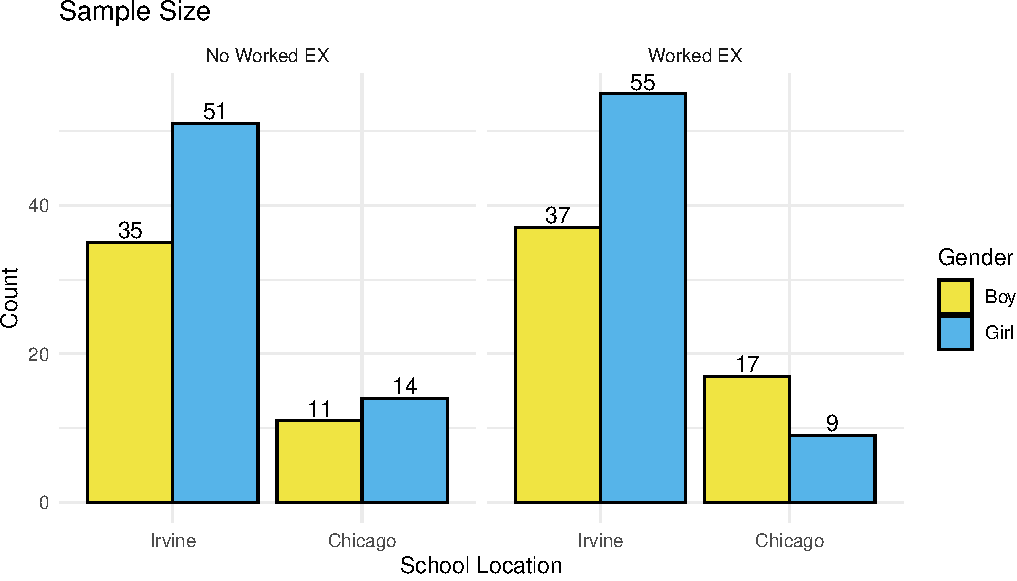
\includegraphics{urop_final_report_files/figure-latex/unnamed-chunk-10-1.pdf}
Based on the regression lines, we see a decrease in students' accuracy
score as their math anxiety scores increase in the no worked example
group (left), and we don't seem much of a change in students' accuracy
scores in the worked example group (right).

\hypertarget{relationship-between-mind-wandering-situational-interest-and-math-anxiety}{%
\subsection{Relationship between mind wandering / situational interest
and math
anxiety}\label{relationship-between-mind-wandering-situational-interest-and-math-anxiety}}

\begin{Shaded}
\begin{Highlighting}[]
\CommentTok{\# MW vs tma}
\NormalTok{mw\_acc1 }\OtherTok{\textless{}{-}}\NormalTok{ dfr }\SpecialCharTok{\%\textgreater{}\%} 
          \FunctionTok{ggplot}\NormalTok{(}\FunctionTok{aes}\NormalTok{(}\AttributeTok{x =}\NormalTok{ mw\_avg, }\AttributeTok{y =}\NormalTok{ TMA\_avg, }\AttributeTok{color =}\NormalTok{ Condition)) }\SpecialCharTok{+}
          \FunctionTok{geom\_point}\NormalTok{() }\SpecialCharTok{+} \FunctionTok{geom\_smooth}\NormalTok{(}\AttributeTok{method =} \StringTok{"lm"}\NormalTok{, }\AttributeTok{se =} \ConstantTok{FALSE}\NormalTok{) }\SpecialCharTok{+}
          \FunctionTok{theme\_bw}\NormalTok{() }\SpecialCharTok{+}
          \FunctionTok{scale\_color\_manual}\NormalTok{(}\AttributeTok{values =} \FunctionTok{c}\NormalTok{(}\StringTok{"\#ef476f"}\NormalTok{,}\StringTok{"\#1b9aaa"}\NormalTok{), }\AttributeTok{labels =} 
                                  \FunctionTok{c}\NormalTok{(}\StringTok{"No Worked EX"}\NormalTok{, }\StringTok{"Worked EX"}\NormalTok{)) }\SpecialCharTok{+}
          \FunctionTok{scale\_fill\_brewer}\NormalTok{(}\AttributeTok{labels =} \FunctionTok{c}\NormalTok{(}\StringTok{"No Worked EX"}\NormalTok{, }\StringTok{"Worked EX"}\NormalTok{)) }\SpecialCharTok{+}
          \FunctionTok{labs}\NormalTok{(}\AttributeTok{x =} \StringTok{"Mind Wandering"}\NormalTok{, }\AttributeTok{y =} \StringTok{"TMA"}\NormalTok{)}
\CommentTok{\#SI vs tma}
\NormalTok{si\_acc1 }\OtherTok{\textless{}{-}}\NormalTok{ dfr }\SpecialCharTok{\%\textgreater{}\%} 
  \FunctionTok{ggplot}\NormalTok{(}\FunctionTok{aes}\NormalTok{(}\AttributeTok{x =}\NormalTok{ SI\_avg, }\AttributeTok{y =}\NormalTok{ TMA\_avg, }\AttributeTok{color =}\NormalTok{ Condition)) }\SpecialCharTok{+}
  \FunctionTok{geom\_point}\NormalTok{() }\SpecialCharTok{+} \FunctionTok{geom\_smooth}\NormalTok{(}\AttributeTok{method =} \StringTok{"lm"}\NormalTok{, }\AttributeTok{se =} \ConstantTok{FALSE}\NormalTok{) }\SpecialCharTok{+}
  \FunctionTok{theme\_bw}\NormalTok{() }\SpecialCharTok{+}
  \FunctionTok{scale\_color\_manual}\NormalTok{(}\AttributeTok{values =} \FunctionTok{c}\NormalTok{(}\StringTok{"\#ef476f"}\NormalTok{,}\StringTok{"\#1b9aaa"}\NormalTok{), }\AttributeTok{labels =} \FunctionTok{c}\NormalTok{(}\StringTok{"No Worked EX"}\NormalTok{, }\StringTok{"Worked EX"}\NormalTok{)) }\SpecialCharTok{+}
  \FunctionTok{labs}\NormalTok{(}\AttributeTok{x =} \StringTok{"Situational Interest"}\NormalTok{, }\AttributeTok{y =} \StringTok{"TMA"}\NormalTok{)}
\CommentTok{\# Side{-}by{-}side plot mw and situational interests with understanding}
\FunctionTok{ggarrange}\NormalTok{(mw\_acc1, si\_acc1, }\AttributeTok{common.legend =} \ConstantTok{TRUE}\NormalTok{, }\AttributeTok{legend=}\StringTok{"bottom"}\NormalTok{, }\AttributeTok{ncol =} \DecValTok{2}\NormalTok{, }\AttributeTok{nrow =} \DecValTok{1}\NormalTok{)}
\end{Highlighting}
\end{Shaded}

\begin{verbatim}
## `geom_smooth()` using formula = 'y ~ x'
\end{verbatim}

\begin{verbatim}
## Warning: Removed 59 rows containing non-finite values (`stat_smooth()`).
\end{verbatim}

\begin{verbatim}
## Warning: Removed 59 rows containing missing values (`geom_point()`).
\end{verbatim}

\begin{verbatim}
## `geom_smooth()` using formula = 'y ~ x'
\end{verbatim}

\begin{verbatim}
## Warning: Removed 59 rows containing non-finite values (`stat_smooth()`).
## Removed 59 rows containing missing values (`geom_point()`).
\end{verbatim}

\begin{verbatim}
## `geom_smooth()` using formula = 'y ~ x'
\end{verbatim}

\begin{verbatim}
## Warning: Removed 70 rows containing non-finite values (`stat_smooth()`).
\end{verbatim}

\begin{verbatim}
## Warning: Removed 70 rows containing missing values (`geom_point()`).
\end{verbatim}

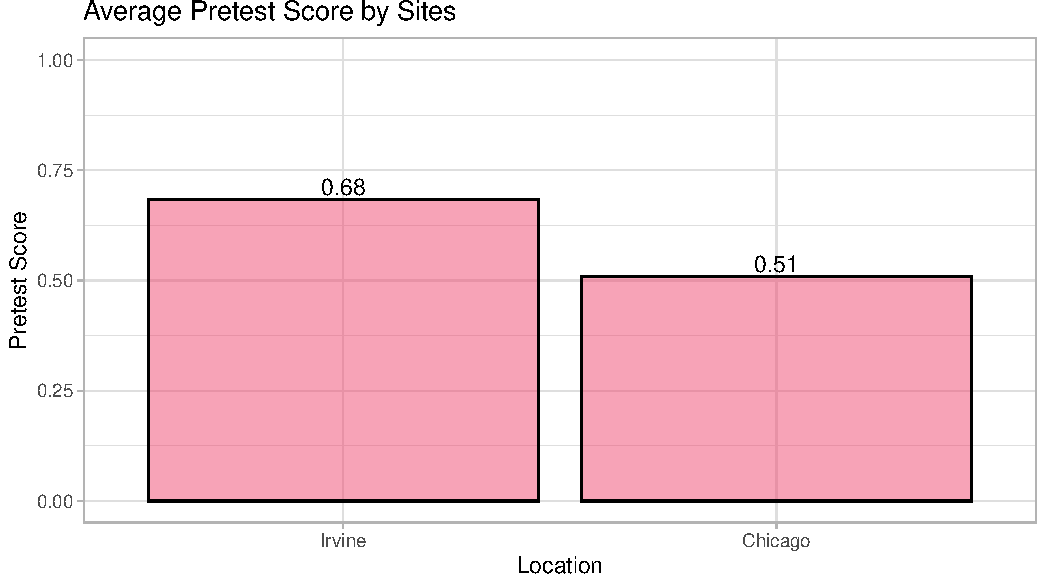
\includegraphics{urop_final_report_files/figure-latex/unnamed-chunk-11-1.pdf}

Based on the regression lines, we see a positive relationship between
mind wandering and math anxiety (left) and a negative relationship
between situational interest and math anxiety (right).

\hypertarget{modeling}{%
\section{Modeling}\label{modeling}}

\hypertarget{predicting-students-achievements-delayed-accuracy-scores}{%
\subsection{Predicting student's achievements (delayed accuracy
scores)}\label{predicting-students-achievements-delayed-accuracy-scores}}

\textbf{Dependent variable:} Post-study accuracy scores
(\texttt{Del\_OverallAcc})

\textbf{Independent variables:} Math anxiety (\texttt{TMA\_avg}),
condition (\texttt{Condition}), interaction term between math anxiety
and condition (\texttt{Condition\ *\ TMA\_avg}), mind wandering avg
(\texttt{mw\_avg}), situational interest (\texttt{SI\_avg})

\begin{Shaded}
\begin{Highlighting}[]
\NormalTok{acc\_fit }\OtherTok{\textless{}{-}}\NormalTok{ df }\SpecialCharTok{\%\textgreater{}\%} 
  \FunctionTok{lm}\NormalTok{(}\AttributeTok{formula =}\NormalTok{ Del\_OverallAcc }\SpecialCharTok{\textasciitilde{}}\NormalTok{ TMA\_avg }\SpecialCharTok{+}\NormalTok{ Condition }\SpecialCharTok{+}\NormalTok{  Condition }\SpecialCharTok{*}\NormalTok{ TMA\_avg }\SpecialCharTok{+}\NormalTok{ mw\_avg }\SpecialCharTok{+}\NormalTok{ SI\_avg) }
\FunctionTok{summary}\NormalTok{(acc\_fit)}
\end{Highlighting}
\end{Shaded}

\begin{verbatim}
## 
## Call:
## lm(formula = Del_OverallAcc ~ TMA_avg + Condition + Condition * 
##     TMA_avg + mw_avg + SI_avg, data = .)
## 
## Residuals:
##      Min       1Q   Median       3Q      Max 
## -0.53186 -0.16809  0.01063  0.17062  0.43554 
## 
## Coefficients:
##                     Estimate Std. Error t value Pr(>|t|)    
## (Intercept)         0.851342   0.096854   8.790 4.08e-16 ***
## TMA_avg            -0.067673   0.028332  -2.389   0.0177 *  
## Condition1         -0.171011   0.081288  -2.104   0.0365 *  
## mw_avg             -0.037099   0.018370  -2.020   0.0446 *  
## SI_avg             -0.005478   0.017012  -0.322   0.7477    
## TMA_avg:Condition1  0.086362   0.037650   2.294   0.0227 *  
## ---
## Signif. codes:  0 '***' 0.001 '**' 0.01 '*' 0.05 '.' 0.1 ' ' 1
## 
## Residual standard error: 0.2209 on 223 degrees of freedom
## Multiple R-squared:  0.06932,    Adjusted R-squared:  0.04845 
## F-statistic: 3.322 on 5 and 223 DF,  p-value: 0.006491
\end{verbatim}

Significant factors for predicting students' accuracy:

\begin{itemize}
\item
  \texttt{TMA\_avg} (\(\beta\) = -0.067673, p = 0.0177): Increased in
  math anxiety caused decrease in students' accuracy
\item
  \texttt{Condition1} (\(\beta\) = -0.171011, p = 0.0365): Worked
  example group had decrease in accuracy by 0.187 percent
\item
  \texttt{mw\_avg} (\(\beta\) = -0.037099, p = 00.0446): Mind wandering
  had negative effect on student's accuracy score. (decrease by
  0.037099)
\item
  \texttt{TMA\_avg:Condition1} (\(\beta\) = 0.086362, p = 0.0227): The
  math anxiety scores of students in worked example group had change in
  accuracy by 0.100 percent -\textgreater{} There is a statistical
  evidence that indicates that effects of math anxiety on accuracy
  scores differ among the study groups
\end{itemize}

Model for worked example group:
\[DelOverallAcc = 0.680331 + 0.018689 * TMAavg - 0.037099 * MWavg - 0.005468 * SIavg\]
Model for no-worked example group:
\[DelOverallAcc = 0.851342 - 0.067673 * TMAavg- 0.037099 * MWavg - 0.005468 * SIavg\]

Math anxiety has different impacts on students' achievements among the
study groups. In worked example group, there is a positive effect on
students' accuracy scores by math anxiety and in no-worked example
group, there is a negative effect on students' accuracy scores by math
anxiety.

\hypertarget{predicting-students-math-anxiety}{%
\subsection{Predicting student's math
anxiety}\label{predicting-students-math-anxiety}}

\textbf{Dependent variable:} Mind wandering avg (\texttt{mw\_avg})

\textbf{Independent variables:} Math anxiety (\texttt{TMA\_avg}),
condition (\texttt{Condition}), interaction term between math anxiety
and condition (\texttt{Condition\ *\ TMA\_avg}), situational interest
(\texttt{SI\_avg})

\begin{Shaded}
\begin{Highlighting}[]
\NormalTok{mw\_fit }\OtherTok{\textless{}{-}}\NormalTok{ dfr }\SpecialCharTok{\%\textgreater{}\%} 
  \FunctionTok{lm}\NormalTok{(}\AttributeTok{formula =}\NormalTok{ mw\_avg }\SpecialCharTok{\textasciitilde{}}\NormalTok{ TMA\_avg }\SpecialCharTok{+}\NormalTok{ Condition }\SpecialCharTok{+}\NormalTok{ TMA\_avg }\SpecialCharTok{*}\NormalTok{ Condition }\SpecialCharTok{+}\NormalTok{ SI\_avg)}
\FunctionTok{summary}\NormalTok{(mw\_fit)}
\end{Highlighting}
\end{Shaded}

\begin{verbatim}
## 
## Call:
## lm(formula = mw_avg ~ TMA_avg + Condition + TMA_avg * Condition + 
##     SI_avg, data = .)
## 
## Residuals:
##     Min      1Q  Median      3Q     Max 
## -1.4683 -0.5322 -0.1488  0.3225  3.1675 
## 
## Coefficients:
##                    Estimate Std. Error t value Pr(>|t|)    
## (Intercept)         1.55264    0.33665   4.612 6.71e-06 ***
## TMA_avg             0.54954    0.09629   5.707 3.61e-08 ***
## Condition1          0.38260    0.29455   1.299   0.1953    
## SI_avg             -0.14973    0.06106  -2.452   0.0150 *  
## TMA_avg:Condition1 -0.28699    0.13559  -2.117   0.0354 *  
## ---
## Signif. codes:  0 '***' 0.001 '**' 0.01 '*' 0.05 '.' 0.1 ' ' 1
## 
## Residual standard error: 0.8034 on 224 degrees of freedom
##   (70 observations deleted due to missingness)
## Multiple R-squared:  0.2282, Adjusted R-squared:  0.2144 
## F-statistic: 16.55 on 4 and 224 DF,  p-value: 6.72e-12
\end{verbatim}

\begin{itemize}
\item
  \texttt{TMA\_avg} (\(\beta\) = 0.54954, p = 3.61e-08): Increase in
  math anxiety cause increase in mind wandering
\item
  \texttt{TMA\_avg:Condition1}(\(\beta\) = -0.28699, p = 0.03540): In
  worked example group, increase in math anxiety cause decrease in mind
  wandering -\textgreater{} There is a statistical evidence indicating
  that effects of math anxiety on mind wandering differ among the study
  groups
\item
  \texttt{SI\_avg} (\(\beta\) = -0.14973, p = 0.0150): Increase in
  situational interest caused decrease in students' mind wandering
\end{itemize}

Model for worked example group:
\[MWavg = 1.93524 + 0.26255 * TMA - 0.14973 * SIavg\]

Model for no-worked example group:
\[MWavg = 1.55264 + 0.54954 * TMA - 0.14973 * SIavg\]

Math anxiety has different impacts on mind wandering among study groups.
Although both groups showed positive effects of math anxiety on mind
wandeirng, in the worked example group, the effect of math anxiety on
mind wandering is smaller than the no worked example group.

\end{document}
